%!TEX program = xelatex+makeindex+bibtex
\documentclass[final]{scrreprt} %scrreprt of scrartcl
\input{../../library/preamble.tex}
\input{../../library/style.tex}
\addbibresource{../../library/bibliography.bib}
\pgfplotsset{yticklabel style={text width=2em,align=right}}
\begin{document}

\chapter{Localization}
\section{Beacon signal}
To pick the optimal beacon signal, it is important to look at the autocorrelation, which is defined as:

\begin{equation}
	R_x(n) = x(-n) * x(n)
\end{equation}

The autocorrelation must ideally be a delta peak to achieve the best matched filter results since the following approximation is used in matched filtering:

\begin{equation}
	x(-n) * y(n) = h(n) * R_x(n) \approx h(n) * \delta (n)
\end{equation}

To define an alternative beacon signal, more criteria were introduced.
Firstly, the first and last bit of the code must be ones and the second and before-last be zeros to have a clear start and ending of the signal.
Secondly, the code must vary enough between zeros and ones, but not in a certain pattern.
This criteria, plus the original criteria of the delta-like autocorrelation resulted in the code \emph{e65a20e5}.
\\ \\
The default autocorrelation is displayed in Figure \ref{fig:default-correlation} and the alternative in Figure \ref{fig:own-correlation}.
The default autocorrelation shows a slimmer autocorrelation, but it contains high peaks around its main peak.
These peaks are way more likely to cause errors because they are almost as high as at the same location as the main peak, causing a relatively lower peak when matched filtering.
For that reason, we allowed more smaller peaks further away from the main peak to reduce the peak height near the main peak.
This way, the main peak is more dominant, likely to result in better matched filter results later on.

\begin{figure}[H]
	\centering
	\setlength\figureheight{4cm}
    	\setlength\figurewidth{0.8\linewidth}
	\input{resources/default-correlation.tikz}
	\caption{Autocorrelation of the default beacon signal.}
	\label{fig:default-correlation}
\end{figure}

\begin{figure}[H]
	\centering
	\setlength\figureheight{4cm}
    	\setlength\figurewidth{0.8\linewidth}
	% This file was created by matlab2tikz v0.4.6 running on MATLAB 8.2.
% Copyright (c) 2008--2014, Nico Schlömer <nico.schloemer@gmail.com>
% All rights reserved.
% Minimal pgfplots version: 1.3
% 
% The latest updates can be retrieved from
%   http://www.mathworks.com/matlabcentral/fileexchange/22022-matlab2tikz
% where you can also make suggestions and rate matlab2tikz.
% 
\begin{tikzpicture}

\begin{axis}[%
width=\figurewidth,
height=\figureheight,
scale only axis,
xmin=0,
xmax=20000,
xlabel={Sample},
ymin=0,
ymax=500,
ylabel={Correlation}
]
\addplot [color=blue,solid,forget plot]
  table[row sep=crcr]{
1	0	\\
46	0	\\
90	0	\\
134	0	\\
178	0	\\
223	0	\\
267	0	\\
311	0	\\
355	0	\\
400	0	\\
444	0	\\
488	0	\\
532	0	\\
577	0	\\
621	0	\\
665	0	\\
709	0	\\
753	0	\\
798	0	\\
842	0	\\
886	0	\\
930	0	\\
975	0	\\
1019	0	\\
1063	0	\\
1107	0	\\
1152	0	\\
1196	0	\\
1240	0	\\
1284	0	\\
1329	0	\\
1373	0	\\
1417	0	\\
1461	0	\\
1505	0	\\
1550	0	\\
1594	0	\\
1638	0	\\
1682	0	\\
1727	0	\\
1771	0	\\
1815	0	\\
1859	0	\\
1904	0	\\
1948	0	\\
1992	0	\\
2036	0	\\
2081	0	\\
2125	0	\\
2169	0	\\
2213	0	\\
2257	0	\\
2302	0	\\
2346	0	\\
2390	0	\\
2434	0	\\
2479	0	\\
2523	0	\\
2567	0	\\
2611	0	\\
2656	0	\\
2700	0	\\
2744	0	\\
2788	0	\\
2833	0	\\
2877	0	\\
2921	0	\\
2965	0	\\
3009	0	\\
3054	0	\\
3098	0	\\
3142	0	\\
3186	0	\\
3231	0	\\
3275	0	\\
3319	0	\\
3363	0	\\
3408	0	\\
3452	0	\\
3496	0	\\
3540	0	\\
3585	0	\\
3629	0	\\
3673	0	\\
3717	0	\\
3761	0	\\
3806	0	\\
3850	0	\\
3894	0	\\
3938	0	\\
3983	0	\\
4027	0	\\
4071	0	\\
4115	0	\\
4160	0	\\
4204	0	\\
4248	0	\\
4292	0	\\
4337	0	\\
4381	0	\\
4425	0	\\
4469	0	\\
4513	0	\\
4558	0	\\
4602	0	\\
4646	0	\\
4690	0	\\
4735	0	\\
4779	0	\\
4823	0	\\
4867	0	\\
4912	0	\\
4956	0	\\
5000	0	\\
5044	0	\\
5089	0	\\
5133	0	\\
5177	0	\\
5221	0	\\
5265	0	\\
5310	0	\\
5354	0	\\
5398	0	\\
5442	0	\\
5487	0	\\
5531	0	\\
5575	0	\\
5619	0	\\
5664	0	\\
5708	0	\\
5752	0	\\
5796	0	\\
5841	0	\\
5885	0	\\
5929	0	\\
5973	0	\\
6017	0	\\
6062	0	\\
6106	0	\\
6150	0	\\
6194	0	\\
6239	0	\\
6283	0	\\
6327	0	\\
6371	0	\\
6416	0	\\
6460	0	\\
6504	0	\\
6548	0	\\
6593	0	\\
6637	0	\\
6681	0	\\
6725	0	\\
6769	0	\\
6814	0	\\
6858	0	\\
6902	0	\\
6946	0	\\
6991	0	\\
7035	0	\\
7079	0	\\
7123	0	\\
7168	0	\\
7212	0	\\
7256	0	\\
7300	0	\\
7345	0	\\
7389	0	\\
7433	0	\\
7477	0	\\
7521	0	\\
7566	0	\\
7610	0	\\
7654	0	\\
7698	0	\\
7743	0	\\
7787	0	\\
7831	0	\\
7875	0	\\
7920	0	\\
7964	0	\\
8008	0	\\
8052	0	\\
8097	0	\\
8141	0	\\
8185	0	\\
8229	0	\\
8273	0	\\
8318	0	\\
8362	0	\\
8406	0	\\
8450	0	\\
8495	0	\\
8539	0	\\
8583	0	\\
8627	0	\\
8672	0	\\
8716	0	\\
8760	0	\\
8804	0	\\
8849	0	\\
8893	0	\\
8937	0	\\
8981	0	\\
9005	30	\\
9043	60	\\
9055	8	\\
9079	7	\\
9110	70	\\
9144	118	\\
9156	22	\\
9158	87	\\
9194	10	\\
9204	19	\\
9216	125	\\
9269	110	\\
9290	19	\\
9295	16	\\
9312	92	\\
9343	33	\\
9360	160	\\
9379	139	\\
9415	22	\\
9444	22	\\
9466	143	\\
9468	37	\\
9499	190	\\
9540	35	\\
9552	155	\\
9564	37	\\
9600	475	\\
9636	37	\\
9648	155	\\
9660	35	\\
9701	190	\\
9732	37	\\
9734	143	\\
9756	22	\\
9785	22	\\
9821	139	\\
9840	160	\\
9866	30	\\
9888	92	\\
9905	16	\\
9910	19	\\
9926	110	\\
9984	125	\\
9996	19	\\
10006	10	\\
10042	87	\\
10044	22	\\
10056	118	\\
10090	70	\\
10116	7	\\
10140	8	\\
10157	60	\\
10195	30	\\
10214	0	\\
10220	0	\\
10264	0	\\
10308	0	\\
10352	0	\\
10397	0	\\
10441	0	\\
10485	0	\\
10529	0	\\
10574	0	\\
10618	0	\\
10662	0	\\
10706	0	\\
10751	0	\\
10795	0	\\
10839	0	\\
10883	0	\\
10928	0	\\
10972	0	\\
11016	0	\\
11060	0	\\
11104	0	\\
11149	0	\\
11193	0	\\
11237	0	\\
11281	0	\\
11326	0	\\
11370	0	\\
11414	0	\\
11458	0	\\
11503	0	\\
11547	0	\\
11591	0	\\
11635	0	\\
11680	0	\\
11724	0	\\
11768	0	\\
11812	0	\\
11856	0	\\
11901	0	\\
11945	0	\\
11989	0	\\
12033	0	\\
12078	0	\\
12122	0	\\
12166	0	\\
12210	0	\\
12255	0	\\
12299	0	\\
12343	0	\\
12387	0	\\
12432	0	\\
12476	0	\\
12520	0	\\
12564	0	\\
12608	0	\\
12653	0	\\
12697	0	\\
12741	0	\\
12785	0	\\
12830	0	\\
12874	0	\\
12918	0	\\
12962	0	\\
13007	0	\\
13051	0	\\
13095	0	\\
13139	0	\\
13184	0	\\
13228	0	\\
13272	0	\\
13316	0	\\
13360	0	\\
13405	0	\\
13449	0	\\
13493	0	\\
13537	0	\\
13582	0	\\
13626	0	\\
13670	0	\\
13714	0	\\
13759	0	\\
13803	0	\\
13847	0	\\
13891	0	\\
13936	0	\\
13980	0	\\
14024	0	\\
14068	0	\\
14112	0	\\
14157	0	\\
14201	0	\\
14245	0	\\
14289	0	\\
14334	0	\\
14378	0	\\
14422	0	\\
14466	0	\\
14511	0	\\
14555	0	\\
14599	0	\\
14643	0	\\
14688	0	\\
14732	0	\\
14776	0	\\
14820	0	\\
14864	0	\\
14909	0	\\
14953	0	\\
14997	0	\\
15041	0	\\
15086	0	\\
15130	0	\\
15174	0	\\
15218	0	\\
15263	0	\\
15307	0	\\
15351	0	\\
15395	0	\\
15440	0	\\
15484	0	\\
15528	0	\\
15572	0	\\
15616	0	\\
15661	0	\\
15705	0	\\
15749	0	\\
15793	0	\\
15838	0	\\
15882	0	\\
15926	0	\\
15970	0	\\
16015	0	\\
16059	0	\\
16103	0	\\
16147	0	\\
16192	0	\\
16236	0	\\
16280	0	\\
16324	0	\\
16368	0	\\
16413	0	\\
16457	0	\\
16501	0	\\
16545	0	\\
16590	0	\\
16634	0	\\
16678	0	\\
16722	0	\\
16767	0	\\
16811	0	\\
16855	0	\\
16899	0	\\
16944	0	\\
16988	0	\\
17032	0	\\
17076	0	\\
17120	0	\\
17165	0	\\
17209	0	\\
17253	0	\\
17297	0	\\
17342	0	\\
17386	0	\\
17430	0	\\
17474	0	\\
17519	0	\\
17563	0	\\
17607	0	\\
17651	0	\\
17696	0	\\
17740	0	\\
17784	0	\\
17828	0	\\
17872	0	\\
17917	0	\\
17961	0	\\
18005	0	\\
18049	0	\\
18094	0	\\
18138	0	\\
18182	0	\\
18226	0	\\
18271	0	\\
18315	0	\\
18359	0	\\
18403	0	\\
18448	0	\\
18492	0	\\
18536	0	\\
18580	0	\\
18624	0	\\
18669	0	\\
18713	0	\\
18757	0	\\
18801	0	\\
18846	0	\\
18890	0	\\
18934	0	\\
18978	0	\\
19023	0	\\
19067	0	\\
19111	0	\\
19199	0	\\
};
\end{axis}
\end{tikzpicture}%
	\caption{Autocorrelation of the alternative beacon signal.}
	\label{fig:own-correlation}
\end{figure}

\section{Matched filter}
\iffalse
A matched filter is used to filter the received audio data from the microphones to the desired signal.
The desired signal will be the beacon signal and the noise that is also present in the received audio data must ideally be removed.
In order to get the noise filtered out, a convolution is used.
This works under the assumption that the desired signal's autocorrelation function is shaped like a delta impulse as described in the previous section.
Since the beacon signal is designed to fit this criterion as much as possible, a reasonable matched filter should be able to be designed.
\\ \\
\fi

\subsection{General}
The matched filter result describes the correlation between the recorded signal from the microphone and the desired signal, which is the beacon signal.
The location in the recorded samples where the beacon signal is most alike the beacon signal will be indicated with a peak.
\\ \\
Ideally, when the noise is completely uncorrelated with the beacon signal and the beacon signal has a delta impulse shaped autocorrelation, the filtered signal consist of only one delta impulse peak at the receival time of the beacon signal at the microphone.
However, this is not entirely the case since there will be correlated noise, a non-ideal beacon signal autocorrelation and beacon signal reflections in the microphone sample data.

\subsection{Reference signal}
The reference signal is used when convolving the sample data.
Multiple references can be used, which will result in different matched filter results.
\\ \\
Firstly, the beacon signal from the refsignal function (refsignal.m) provided via BlackBoard can be used directly.
When using this reference signal in Appendix \ref{app:code}:matched-filter.m, the results from Figure \ref{fig:orgref} were found.
This however does not perform very well since the peaks are not clear at larger distances.
Only the close recording of the third microphone with proportionally few noise produces a reasonable peak as indicated in the left with the red indicator close to the correct location.
At larger distances, even the unfiltered signal is better than the filtered signal.
\\ \\
Secondly, the recording of the beacon signal at about 10 cm can be used.
The distance of 10 cm is picked because at larger distances the noise is proportionally larger and at lower distances the microphone might clip.
This measurement takes the channel distortions of the beacon, 10 cm air and microphone into account.
Therefore, this reference signal will look much more like the captured one in the received microphone sample data, which will result in clearer peaks when convolving.
The results of the measured beacon signal as reference is displayed in Figure \ref{fig:no-toep}, for which Appendix \ref{app:code}:matched-filter.m was used again.
The peaks are detected correctly, as read from the red indicators in the left plots.

\subsection{Convolution type}
When convolving, two types of convolution can be used: linear convolution or circular convolution.
Previously, only linear convolution was used, but it can be more efficient to use the circular variant.
This is the case when multiplying with the Toepitz matrix, which equals the circular convolution of the two multiplied matrices.
Unlike linear convolution, matrix multiplication can be performed efficiently in C\#.
\\ \\
Circular convolution is however not exactly the same as linear convolution.
The edges of the convolved signal are tied together, resulting in distortion at the edges of the result.
The area of this distortion depends of the size of the signal which is being convolved with.
When this signal is relatively long, the distorted area is long as well on both sides of the result.
The result when performing a circular convolution using a Toupitz matrix with Appendix \ref{app:code}:matched-filter-toep.m is displayed in Figure \ref{fig:toep}.
\\ \\
As seen in Figure \ref{fig:toep}, the peaks are not as clear as in Figure \ref{fig:no-toep} where linear convolution was used.
Therefore, the linear convolution is preferred.
When using the linear convolution, the processing time must be kept in mind as well, but this was taken care of by multi-threading.

\section{TDOA Localization}
For our car two TDOA estimation algorithms are implemented.
The algorithms were developed simultaneously and supplement each other as sometimes the first algorithm might produce a 'NaN'.

\subsection{First algorithm}
Before going into TDOA estimation, it was assumed that the time it took for the sound to travel from the beacon to all microphones was known.
This made the calculation a lot easier since it can be solved using two microphones only.
\\ \\
Figure \ref{fig:location} shows how the location of the car can be found when the locations of the microphones (and thus the distance between them, $a_1 + a_2$) and the time between transmission and arrivals at the two microphones $t_1$ and $t_2$, which can be converted into a distance using the speed of sound $c \approx \SI{343.2}{\metre\per\second}$.
Using this information, two possible locations can be found, the real location of the car and its mirrored version over the line between the two microphones as shown in Figure \ref{fig:location} as the dotted lines.

\begin{figure} [H]
\centering
	\begin{tikzpicture}	
		\node [anchor=east] at (0,0) (mic1) {Mic 1};
		\node [anchor=west] at (9,0) (mic2) {Mic 2};
		\node [anchor=south] at (6,3) (car) {Beacon};
		\node [anchor=north] at (4.5,-0.25) (a) {$a$};

		\draw (0,0) -- node[below]{$a_1$} (6,0)
			-- node[left]{$x$} (6,3)
			-- node[above, sloped]{$t_1 c$} (0,0);

		\draw (6,0) -- node[below]{$a_2$} (9,0)
			--  node[above, sloped]{$t_2 c$} (6,3);

		\draw [dotted] (0,0) -- (6,0)
			-- (6,-3)
			-- (0,0);

		\draw [dotted] (6,0) -- (9,0)
			--  (6,-3);
	\end{tikzpicture}
	\caption{Location determination.}
	\label{fig:location}
\end{figure}

From Figure \ref{fig:location}, the following equations can be formulated:
\begin{equation}
	a_1 = \frac{t_1^2 c^2 - t_2^2 c^2 + a^2}{2 a}
\label{eq:a1}
\end{equation}

\begin{equation}
	x = \sqrt{t_1^2 c^2 - a_1^2}
\end{equation}

To find the absolute location of the beacon on the field when Mic 1 and Mic 2 are not necessarily on the same y-coordinate, an angular translation is needed as illustrated in Figure \ref{fig:angular-translation}.

\begin{figure} [H]
\centering
	\begin{tikzpicture}	
		\node [anchor=east] at (0,0) (mic1) {Mic 1};
		\node [anchor=south east] at (2.1213,6.3439) (car) {Beacon};
		\node [anchor=south west] at (1,0.15) {$\theta$};

		\draw [-*] (0,0) -- node[below]{$a_1$} (6,0)
			-- node[left]{$x$} (6,3);

		\draw [dashed, -*] (0,0) -- (4.2426,4.2426)
			-- (2.1213,6.3439);

		\draw [->] (1,0) arc (0:45:1);
	\end{tikzpicture}
	\caption{Angular translation.}
	\label{fig:angular-translation}
\end{figure}

With $\theta$ the angle between Mic 1 and Mic 2:

\begin{equation}
	\theta = -\arctan{\frac{\text{Mic 2}_y - \text{Mic 1}_y}{\text{Mic 2}_x - \text{Mic 1}_x}}
\end{equation}

The beacon location in x- and y-coordinates are found by adding the point ($a_1$, $x$) with angular translation of $\theta$ to the location of Mic 1.
\\ \\
Since five microphones will be used instead of just two, the mirrored versions can be filtered out, leaving only the real location of the car as a solution.
By using only two microphones per location estimation instead of all five at once, wrong arrival times can be filtered out easily.
However, when the arrival times are all poorly defined due to errors, it might not be possible to filter the mirror images out of the solution sets.

\subsection{Height correction}
The height difference between the audio beacon and the microphones causes a larger time delay than expected when only looking at the 2D plane only.
However, this time delay can be corrected using Pythagoras' theorem:

\begin{equation}
	t_{2D} = \sqrt{t_{3D}^2 - \Delta h^2}
\end{equation}

With $\Delta h$ the height difference between the beacon and the microphone.
The resulting $t_{2D}$ can be used in the basic localization to exactly calculate the beacon location, independent of the height difference.

\subsection{TDOA to arrival times}
In order to use the TDOA data in the algorithm mentioned above, the time delays between the transmission and reception of the signal per microphone must be calculated from the TDOA data.
For this, it is known that this transition from TDOA to time delays is accomplished by adding a the same time constant time difference per microphone.
This constant is defined as the time difference between the absolute time of transmission and the absolute start time of the sample data, e.g. the absolute time of sample number one.
\\ \\
To find this constant, an orthogonal base of three microphones is used as in Figure \ref{fig:constant}.

\begin{figure} [H]
\centering
	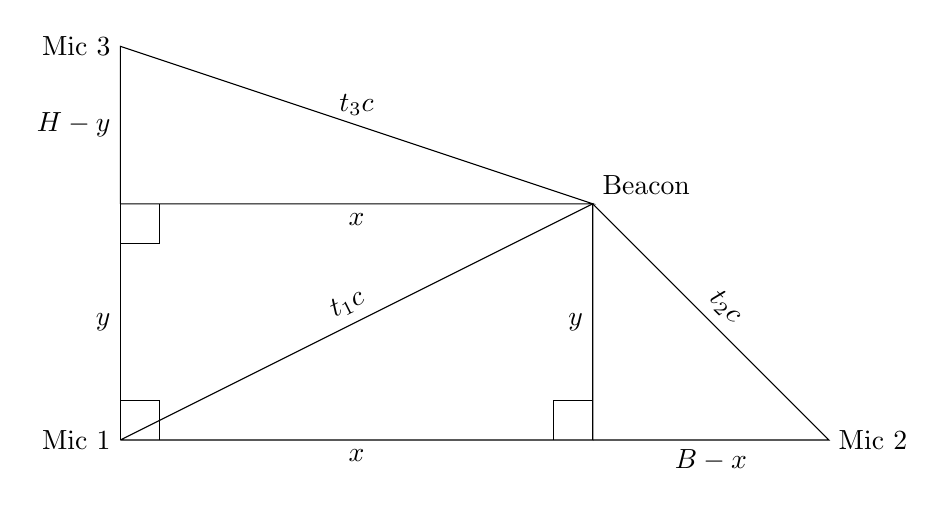
\begin{tikzpicture}	
		\node [anchor=east] at (0,0) (mic1) {Mic 1};
		\node [anchor=west] at (9,0) (mic2) {Mic 2};
		\node [anchor=east] at (0,5) (mic1) {Mic 3};
		\node [anchor=south west] at (6,3) (car) {Beacon};

		\draw (0,0) -- node[below]{$x$} (6,0)
			-- node[left]{$y$} (6,3)
			-- node[above, sloped]{$t_1 c$} (0,0);

		\draw (6,0) -- node[below]{$B - x$} (9,0)
			--  node[above, sloped]{$t_2 c$} (6,3);

		\draw (0,0) -- node[left]{$y$} (0,3);

		\draw (0,3) -- node[left]{$H - y$} (0,5)
			-- node[above]{$t_3 c$} (6,3)
			-- node[below]{$x$} (0,3);

		\draw (0.5,0) -- (0.5,0.5) -- (0,0.5);
		\draw (5.5,0) -- (5.5,0.5) -- (6,0.5);
		\draw (0,2.5) -- (0.5,2.5) -- (0.5,3);
	\end{tikzpicture}
	\caption{Model used for determination of the constant time error.}
	\label{fig:constant}
\end{figure}

Using the formula of the altitude of a triangle, e.g. $y$ in triangle (Mic 1, Mic 2, Beacon), the altitude is defined as:

\begin{equation}
	y = \frac{2 \sqrt{s(s - B)(s - D_1)(s - D_2)}}{B}
\label{eq:y1}
\end{equation}

With $B$ the base of the triangle, $D_1$ and $D_2$ the other two sides of the triangle and $s$ half of the perimeter of the triangle, $s = (B + D_1 + D_2) / 2$.
In the case of triangle (Mic 1, Mic 2, Car) with altitude line $y$, the base $B = \lVert Mic 1 - Mic 2 \rVert$ and the other two sides as $D_1 = t_1 c$ and $D_2 = t_2 c$ or vice versa.
\\ \\
For triangle (Mic 1, Mic 3, Car), $y$ is defined by:

\begin{equation}
	y = \frac{t_1^2 c^2 - t_3^2 c^2 + H^2}{2 B}
\label{eq:y2}
\end{equation}

The parameters $t_1$, $t_2$ and $t_3$ are defined with an offset of the constant we wish to find.
Using Equation \ref{eq:y1} and \ref{eq:y2}, which are defined to the same $y$ since the three microphone form an orthogonal basis, and having an additive constant to $t_1$, $t_2$ and $t_3$, Matlab calculated the formula of the constant using the script report6-2.m from Appendix \ref{app:code}.
\\ \\
Now that the constant is known, the algorithm using two microphones and the arrival times can be applied.
It must however be noted that the height difference between the microphones and the beacon is not applied to the calculation of the constant time.
Matlab could not find an explicit solution for the 3D situation, hence it was not included.
This will lead to an error in the resulting location.
However, the error will be very small when the beacon is not close by the microphone, hence only one microphone can be compromised at once.
For that, the base of orthogonal microphones shift to all four possible combinations and check for the best basis with the least standard deviation between the subresulting locations.
\\ \\
The final Matlab script can be found in Appendix \ref{app:code}: location.m, which implements everything discussed so far in this chapter.

\subsection{Testing with test data}
\label{sec:testing}
The test script location-errors.m as found in Appendix \ref{app:code} was used to find the error mean, standard deviation and maximum.
The first test was in 2D mode; all microphones and the beacon were on the same height.
\\ \\
The other tests were with the four surrounding microphones 10 cm higher than the beacon and the last microphone 65 cm higher than the beacon.
The five microphones were set up as in the five microphone test setting from Labday 5.
All tests were done by calculating 2.500 points linearly spread on the 2.9m x 2.9m field.
The results are displayed in Table \ref{tab:errors}.

\begin{table} [H]
\centering
	\begin{tabular}{ c | c | c | c }
  	Setup & Error mean (mm) & Error standard deviation (mm) & Max error (mm) \\ \hline
  	2D & 0 & 0 & 0 \\
  	3D without height correction & 31.2 & 10.9 & 61.8 \\
	3D with height correction & 3.4 & 2.4 & 13.6 \\
	\end{tabular}
\caption{Location error details for different setups.}
\label{tab:errors}
\end{table}

It can be concluded that the algorithm works with sufficient accuracy since the error mean and maximum are low enough for accurate location estimation.
More than 1 cm accuracy is indeed not needed for the purpose of the project.
The height correction definitely adds accuracy to the location estimation as expected, hence it will be used later on.
This is however when the TDOA information is nearly infinitely accurate, which will not be the case.

\subsection{Testing with non-ideal data}
Errors will occur when the estimated speed of sound is not exactly correct since it varies with environment parameters such as temperature, humidity and air pressure.
Using the test script from the previous subsection \ref{sec:testing} with an altered speed of sound with the input data generation, a certain error will occur.
This was tested for the range of 1 to 5 percent deviation from the actual speed of sound, the results are shown in Table \ref{tab:c-errors}.

\begin{table} [H]
\centering
	\begin{tabular}{ c | c | c | c }
  	Deviation in speed of sound (\%) & Error mean (cm) & Error standard deviation (cm) & Max error (cm) \\ \hline
  	1 & 1.39 & 0.62 & 2.89 \\
	2 & 1.45 & 0.65 & 3.02 \\
	3 & 2.54 & 1.18 & 5.40 \\
	4 & 3.60 & 1.68 & 7.54 \\
  	5 & 3.12 & 1.09 & 6.18 \\
	\end{tabular}
\caption{Location error details for various deviations of the speed of sound.}
\label{tab:c-errors}
\end{table}

Besides errors in the speed of sound, errors will occur in determining the arrival times at the microphones.
These errors can be simulated using a normal distribution with varying standard deviations, the results are displayed in Table \ref{tab:std-errors}.
The noise standard deviation can be converted to standard deviation in distance by multiplying with the speed of sound.
At \SI{0.15}{\milli\second}, which corresponds to \SI{5.1}{\centi\metre}, about \SI{5}{\centi\metre} accuracy is achieved.

\begin{table} [H]
\centering
	\begin{tabular}{ c | c | c | c }
  	Noise standard deviation (\si{\milli\second}) & Error mean (\si{\centi\metre}) & Error standard deviation (\si{\centi\metre}) & Max error (\si{\centi\metre}) \\ \hline
	0.1 & 3.34 & 1.88 & 11.88 \\
	0.15 & 4.90 & 2.97 & 50.51 \\
	0.2 & 6.70 & 5.00 & 125.76 \\
	0.3 & 11.34 & 9.02 & 127.42 \\
	0.4 & 16.35 & 13.55 & 180.23 \\
	0.5 & 23.03 & 21.88 & 292.76 \\
	\end{tabular}
\caption{Location error details for various arrival time error standard variations.}
\label{tab:std-errors}
\end{table}

\iffalse
\begin{table} [H]
\centering
	\begin{tabular}{ c | c | c | c }
  	Noise standard deviation (\si{\milli\second}) & Error mean (\si{\milli\metre}) & Error standard deviation (\si{\milli\metre}) & Max error (\si{\milli\metre}) \\ \hline
  	0.1 & 10.0 & 5.5 & 35.9 \\
	0.2 & 19.2 & 9.9 & 57.0 \\
	0.3 & 27.8 & 14.9 & 92.6 \\
	0.4 & 36.5 & 19.5 & 111.8 \\
  	0.5 & 46.2 & 24.0 & 147.4 \\
	0.6 & 56.3 & 30.4 & 347.8 \\
	0.7 & 67.9 & 42.6 & 544.3 \\
	0.8 & 80.7 & 55.3 & 847.4 \\
	0.9 & 94.8 & 67.4 & 958.9 \\
	1.0 & 
	\end{tabular}
\caption{Location error details for various deviations of the speed of sound.}
\label{tab:errors}
\end{table}
\fi

\subsection{Testing with real measurement data}
The test with five microphones, four in a \SI{2.9}{\metre} x \SI{2.9}{\metre} square on \SI{38}{\centi\metre} height and one microphone placed \SI{2.4}{\metre} from the center of the square on \SI{0.93}{\centi\metre} high.
The car was placed on seven defined spots on the field, the first five at all microphones, the sixth at the center of the square and the last \SI{1}{\metre} towards a corner of the square.
The recordings from the microphones were saved to be processed later on using the matched filter.
The results are shown in Figure \ref{fig:map}.
\\ \\
On this map all microphones and other test points are shown as dots and the calculated locations as crosses.
The five measurements at the microphones are not the exact places since the car could not come very close to the microphones, so the car was placed about 5 cm from the microphones toward the center of the room.
The microphone outside the square could not be localized, this is because the algorithm is made to work inside the square of microphones.
The algorithm fails when calculating the constant time offset, which becomes imaginary.
This will likely not be a problem since the car will stay inside the square in practice.
\\ \\
The error in the localization is less than \SI{5}{\centi\metre}, also because the exact location of the car was not known since the car is rather large.
All together it can be concluded that the localization works with sufficient accuracy in practice too.

\begin{figure} [H]
\centering
	\begin{tikzpicture}	
		%\node [anchor=south] at (0,0) (mic1) {Mic 1};

		\fill[black,thick] (0, 0) circle [radius=0.5mm];
		\fill[black,thick] (0, 2.9*2) circle [radius=0.5mm];
		\fill[black,thick] (2.9*2, 2.9*2) circle [radius=0.5mm];
		\fill[black,thick] (2.9*2, 0) circle [radius=0.5mm];
		\fill[black,thick] (-1.05*2, 1.45*2) circle [radius=0.5mm];
		\fill[black,thick] (1.45*2, 1.45*2) circle [radius=0.5mm];
		\fill[black,thick] (1.45*2 + 0.707*2, 1.45*2 + 0.707*2) circle [radius=0.5mm];

		\draw (0.0014*2 + 0.1, 0.0810*2 + 0.1) -- (0.0014*2 - 0.1, 0.0810*2 - 0.1);
		\draw (0.0014*2 + 0.1, 0.0810*2 - 0.1) -- (0.0014*2 - 0.1, 0.0810*2 + 0.1);

		\draw (0.0435*2 + 0.1, 2.8779*2 + 0.1) -- (0.0435*2 - 0.1, 2.8779*2 - 0.1);
		\draw (0.0435*2 + 0.1, 2.8779*2 - 0.1) -- (0.0435*2 - 0.1, 2.8779*2 + 0.1);

		\draw (2.8450*2 + 0.1, 2.9414*2 + 0.1) -- (2.8450*2 - 0.1, 2.9414*2 - 0.1);
		\draw (2.8450*2 + 0.1, 2.9414*2 - 0.1) -- (2.8450*2 - 0.1, 2.9414*2 + 0.1);

		\draw (2.8536*2 + 0.1, 0.0276*2 + 0.1) -- (2.8536*2 - 0.1, 0.0276*2 - 0.1);
		\draw (2.8536*2 + 0.1, 0.0276*2 - 0.1) -- (2.8536*2 - 0.1, 0.0276*2 + 0.1);

		\draw (1.4312*2 + 0.1, 1.4258*2 + 0.1) -- (1.4312*2 - 0.1, 1.4258*2 - 0.1);
		\draw (1.4312*2 + 0.1, 1.4258*2 - 0.1) -- (1.4312*2 - 0.1, 1.4258*2 + 0.1);

		\draw (2.1686*2 + 0.1, 2.2024*2 + 0.1) -- (2.1686*2 - 0.1, 2.2024*2 - 0.1);
		\draw (2.1686*2 + 0.1, 2.2024*2 - 0.1) -- (2.1686*2 - 0.1, 2.2024*2 + 0.1);
	\end{tikzpicture}
	\caption{Map with errors.}
	\label{fig:map}
\end{figure}

\subsection{Second algorithm}
Assuming a known distance difference $\Delta_{01}$ between two microphones $R_{0} (x_{0},y_{0})$ and $R_{1} (x_{1},y_{1})$ the following equation can be formed:
\begin{equation}
\Delta_{01} = \left| \sqrt{(x_0-x_e)^2+(y_0-y_e)^2} - \sqrt{(x_1-x_e)^2+(y_1-y_e)^2)}\right|
\end{equation}
Because the positions of the microphones are known there are two unknowns, $x_e$ and $y_e$.
With sufficient equations, meaning more microphones, the unknown values can be found.
Using the steps from tutorial 6 in the EPO4 manual we end up with a set of equations of the form $Ay=b$ which can be solved for $y$ which contains the unknown variables.
This method is implemented with five microphones.
The algorithm proofed to be less accurate than the first algorithm with an accuracy of about \SI{8}{\centi\metre}.
%
\end{document}
